\section{{\bf PLAN}}
{\bf About the ACMS program}

The ACMS {\em (Applied and Computational Mathematical Sciences)} was
introduced in \mmp{fill} as a joint undergraduate program between the
departments of Applied Mathematics, Computer Science and Engineering,
Mathematics and Statistics, among others.

The ACMS program is structured into a {\em core}, totaling 43 credits,
and a set of options, or {\em tracks}. The same set of core courses is
required for all options (with some exceptions). Options are either
associated with a particular application domain (Biological and Life
Sciences, Mathematical Economics, Social and Behavioral Sciences,
Engineering and Physical Sciences) or with a particular area of
specialization in the mathematical sciences ({\em Discrete Math and
  Algorithms, Operations Research, Scientific Computing and Numerical
  Analysis, and Statistics}). 

During the recent academic year, the enrollment in ACMS has been at
about 200 (what? student/year?), divided as follows: 


It is the Statistics track of ACMS that we are aiming to tranform. Currently, this track contains, in addition to the core courses (43 credits), the followin

{\bf Option Core (37 credits)}
\bit
    \item PHYS 121, 122, 123 (5,5,5) (can be replaced by courses in another application area)
    \item STAT 302: (2) Statistical Software and Its Applications R
    \item STAT 340: (4) Introduction to Probability and Mathematical Statistics
    \item STAT 341,342: (4,4) Introduction to Probability and Statistical Inference I,II
    \item STAT 421: (4) Applied Statistics and Experiment Design
    \item STAT 423: (4) Applied Regression and Analysis of Variance
\eit
{\bf Option Electives (10 credits)}
\bit
    \item MATH/STAT 396: Probability III
    \item MATH/STAT 491, 492: Introduction to Stochastic Processes
\item[]
    \item STAT 403: (3) Introduction to Resampling Inference
    \item STAT 427: (3) Introduction to Analysis of Categorical Data
    \item STAT/BIOST 529: (3) Sample Survey Techniques
\item[]
    \item CSE 373 (3) Data Structures
\item[]
    \item MATH 300: (3) Mathematical Reasoning
    \item MATH 327: (3) Introductory Real Analysis I
    \item MATH 407,408,409: (3,3,3) Linear, Nonlinear,\& Discrete Optimization
\item[]
    \item STAT 428: (4) Multivariate Analysis for the Social Sciences
    \item GEOG 426: (5) Quantitative Methods in Geography
    \item QMETH 528: (4) Survey Sampling Applications
\eit
The program web page recommends that ``[this track] is ideally suited as a second major for students with a primary focus in the biological sciences, earth sciences, social sciences, engineering, or management science.''

De facto, the track curricullum differs little, most notably by the
presence of the computer programming class CSE 142, from the
``standard'' Statistics major. Another notable difference from the
statistics major is STAT 390, a class for non-majors. 

To note also that the enrollment in the ACMS Statistics track was
\mmp{fill} in the last years, while the enrollment in the Statistics
major is at an all times high, with \mmp{fill}.

We will transform this track into a Computationally Minded Statistics
Major. In other words, we do not aim to produce scientists who also
know statistics (which can be well served by the other tracks of ACMS)
but full-fledged statisticians who can function autonomously in the
cyberworld.

 There are several motivating factors:
\bit
\item Interest in statistics is at an all times high, as witnessed by our enrollment numbers. We expect that the ACMS Statistics track will be as well.
\item The role of the statistician as data analyst has become both
  more central, and more demanding. As more data analysis and more
  decisions based on it are being shifted from humans to computers,
  statistics is called upon to design and validate the procedures used
  to take these decisions. Thus, the statician's importance in a much
  wider range of human activities, be they science or buisness. But
  the statistician's responsability is comensurately growins, as she
  needs to master the skills required by cyber-enabled science and
  data analysis. 
\item These skills include are not limited to computer using and
  programming skills. The nature of statistical analyses itself is
  affected \mmp{get some citations} as it has been long
  recognized. Computationally aware statistical methods need to be
  designed. Very large samples will support models of a complexity
  that could not be considered in real-life scenarios a decade or two
  ago. It is now not possible to perform model selection by explicitly
  comparing all possible models (i.e. there can be an exponential
  number of models to compare) and regularization methods are often
  called into play, as are approximate computational
  techniques. Leveraging unlabeled data for prediction is now an
  almost universal necessity. Devising new methods to evaluate complex
  models in an environment that is not stationary, nor controlled are
  some of the challenges of modern data analysis.
\item The proposal fits in and leverages other efforts and successes at UW in creating a strong collaborative environment for \cdse~ (the e-science Institute, the IGERT for graduate education in Big Data and related PhD tracks already existing in CSE and Statistics). The time is ripe to involve undergraduates, and specifically statistics and mathematics majors in this change.
\item This proposal is in the spirit of the ACMS original mission,
  bringing this part up to speed with the demands of the coming decade.
\eit

{\bf Why this particular approach} Currently, computer education is
assured primarily through two core courses, CSE 142, 143
\cite{cse142}. These set the foundations in the understanding of
computer programming, but they are of a general nature, and are mainly
focuses towards preparing future programmers. (These courses are the
same courses that the about 500 CSE majors take). Thus, there is no
room for data analysis applications in these courses. The need for a
dedicated scientific computing course was recognized, hence the
Scientific Computing track and courses developed by AMATH. There is an
R course (STAT 302, 2 credits) offered as an elective. However, for
reasons we will develop later, we consider that Python is the more
appropriate computer language for our goals. Thus, we will both
introduce Python and will use it to teach statitical methodology. As
Python will be taught as a second programming language, and as it is
similar enough to Java, we expect the students to be assimilate it
quickly under our guidance. 

\mmp{ to continue after the proposal more fleshed out}

{\bf What we want to do}

\bit
\item To transform the ACMS Statistics track into a computer intensive statistics major. 
  \bit
   \item Stage 1: Design and introduce two new courses STAT 391, ASTRO 598 as {\em electives} in the track.
   \item Stage 2: Redesign the track: move STAT 391, Stochastic Processes STAT 481, 482 into the core. As this will no longer be regarded as a second major for science students, we will make room by removing the PHYS 121, 122, 123 courses (15 credits) from it. Reorganizing the electives into two groups: group I (math/stat electives) and group II computing and science electives. 
   \item Stage 3: ?? Making these courses accessible to mathematics majors, via William Steins python programming course. 
  \eit
\item To develop a software infrastructure for teaching \cdse~ in
  Python. This will include data sets, data analysis problems,
  software libraries, and course modules built around the data and
  problems. This infrastructure will be made available via the
  web. Due to its modular structure, it will be useable as needed by
  instructors in other courses.
\item To organize an Undergraduate Research Seminar. In this seminar, unlike the ACMS 
\item To organize a 3 day workshop for instructors in statistics and related fields that will teach the basics of using our sofware infrastructure and will impart our experience in the project.
\eit



\comment{
The Program Core is a set of courses totaling 43 credits which are generally required for all ACMS majors. Exceptions are specifically pointed out in the descriptions of the various options. The core courses will provide a solid foundation from which students may pursue any of the approved degree pathways within the Program. }

\mmp{put this somewhere?}
{\em A fundamental concept at the core of the ACMS program is modeling - casting a real world problem in a way that makes it amenable to mathematical, statistical, or computational analysis. 
 Continuous modeling, while central to many applications, is not part of the CSE undergraduate curriculum, and statistical modeling is only a small component. }





\subsection{ASTR 490} 

Was it 490? Andy remembers...


Copied text from that email, which was copied from our book, to see
how many pages it would take...

\subsubsection{Motivation for Astr 490}

Astronomy and astrophysics are witnessing dramatic increases in data volume 
as detectors, telescopes, and computers become ever more powerful. During the 
last decade, sky surveys across the electromagnetic spectrum have collected 
hundreds of terabytes of astronomical data for hundreds of millions of sources. 
Over the next decade, the data volume will enter the petabyte domain, and provide 
accurate measurements for billions of sources. Astronomy and physics students 
are not traditionally trained to handle such voluminous and complex data sets. 
Furthermore, standard analysis methods employed in astronomy often lag far 
behind rapid progress in statistics and computer science. The main
goal of this course is to contribute to efficient training of next
generations of students to 
handle the fast growing data sets, not only in astronomy, but in other quantitative 
sciences as well. 

This course will be aimed at physical and data-centric math,
statistics, science and engineering students
who have an understanding of the science drivers for analyzing large data sets but 
may not be aware of appropriate statistical techniques for doing so. The course work 
will provide to students a connection between scientific data analysis problems and 
modern statistical methods. We will limit theoretical discussions to the minimum 
required to understand the algorithms and will build the courses upon an 
example-driven compendium of modern statistical and data mining methods, 
together with carefully chosen examples based on real modern data sets, and of 
current astronomical applications that will illustrate each method introduced in the 
book. Discussion of the advanced material will be supported by appropriate (publicly 
available) Python code and data which will enable students to perform exercises, 
evaluate the techniques, and adapt them to their own fields of interest. We chose to 
use Python, a powerful and flexible programming language that is quickly becoming 
a standard in data-intensive sciences (and elsewhere). 

The target audience for our course includes undergraduate students with scientific 
or engineering background, but it is likely that graduate students
would benefit from it too. Familiarity with calculus and other basic mathematical 
techniques will be assumed, but no extensive prior knowledge in statistics will be 
required. 

The course outline: 

\begin{enumerate} 
\item Computational Challenges in data-intensive astronomy and astrophysics
\begin{itemize}
\item  data types and data management systems 
\item  analysis of algorithmic efficiency
\item  types of computational problems and strategies for speeding them up 
\item  data visualization challenges
\item  selection effects and truncated/censored data in astronomical context 
\end{itemize}
\item Searching for structure in astronomical point data
\begin{itemize}
\item  non-parametric density estimation
\item  nearest-neighbor density estimation
\item  parametric density estimation
\item  finding clusters in data 
\item  correlation functions 
\end{itemize} 
\item Dimensionality reduction
\begin{itemize}
\item  principal component analysis in astronomical context
\item  non-negative matrix factorization 
\item  independent component analysis and projection pursuit 
\item  manifold learning
\end{itemize} 
\item Regression and model fitting
\begin{itemize}
\item  regresion for linear models
\item  non-linear regression
\item  kernel and principal component regression
\item  methods for handling heteroscedastic and non-Gaussian errors 
\item  Gaussian processes
\item  overfitting, underfitting and cross-validation
\end{itemize} 
\item Classification 
\begin{itemize}
\item  generative classification methods
\item  discriminative classification method 
\item  evaluation and comparison of classifiers: ROCcurves 
\end{itemize} 
\item Time series analysis in astronomy
\begin{itemize}
\item  main concepts and tools for time series analysis
\item  analysis of periodic time series 
\item  temporally localized signals
\item  analysis of stochastic processes
\end{itemize} 
\end{enumerate} 


We will textbook {\it ``Statistics, Data Mining, and Machine Learning in Astronomy:
A Practical Python Guide for the Analysis of Survey Data''} (Princeton Series in Modern 
Observational Astronomy) coauthored by Co-PIs on this prooposal. 


\subsection{Python Packages} 



We will leverage all the publicly available modern python tools. 
In particular,  seminar work will be built around the {\it astroML} package
that was developed to support textbook to be used with the proposed course. 


\begin{figure*}[!t]
\vskip -5.5in
\includegraphics[width=1.02\hsize,clip]{astroML.eps}
\vskip -2.0in
\caption{We will leverage all the modern python tools available in {\it astroML} and
other packages.} 
\label{Fig:astroML}
\end{figure*}




\subsection{Workshop} 


At the last meeting, we assumed a 3-day workshop for about 30 faculty from other institutions
of higher learning who would want to emulate our program. Further assuming \$20/day/person
for lunch and coffee, and \$75/person for conference dinner, \$1,500 for the workshop venue,
and four grants of \$500 to young faculty and postdocs, we need about \$7,500 for the workshop. 



\subsection{Budget} 

We assumed a 3-year long project. 

We assumed 2.5 months of summer salary for Marina, and a postdoc. About \$150,000/year. 

We assumed 1 month of summer salary for both \v{Z}I and Andy to demonstrate seriousness,
and a graduate student. About \$100,000/year. 

All together, about \$750,000 for 3 years. If this is above the limit, perhaps we could 
descope faculty to only the first two years? 



